\chapter{Introduction}
Medical and biological image analysis usually is a time-consuming task that can only be carried out by domain experts. However, the sheer amount of data produced in experiments has become hard to handle manually, requiring computer-based assistance or even completely automatic image segmentation algorithms.\\

\noindent This thesis deals with the special case of automatically identifying and marking different parts of cells in images that were created using a form of fluorescence microscopy, called \textit{Spinning Disk Confocal Microscopy}. The cells in question are macrophage cells of the common fruit fly, \textit{Drosophila melanogaster}, which has long been a research subject in biological experiments because of its suitability as an animal for biological testing. The migration and shape of these cells are of particular biological interest. To obtain images of these cells while they are still alive (\textit{in vivo}), the macrophages are genetically altered so that they include \textit{green fluorescent protein}, which emits green light when excited by blue or ultraviolet light. This fluorescence response is then filtered and used to create an image, or even a series of images to show the movement of these cells in form of a video. These microscopy images contain four regions of interest: The background, containing no cell material, the cell body, the \textit{Lamellipodium} and the \textit{Filopodia}. The latter two terms describe part of the cytoplasm of a cell, which can be exuded from the cell body in the form of a broad, translucent area, the Lamellipodium, and long, thin spikes traversing the Lamellipodium and the space beyond it, the Filopodia. These cell parts play roles in cell movement during wound healing and cell infection. Even for human experts, correctly identifying these areas is not always possible. Unfortunately, the stained samples are sensitive to light: if the samples are illuminated for too long, they deteriorate and become unusable. Also, samples are often stacked while performing microscopy to create 3D models. When viewed as individual 2D images, these circumstances lead to images that are often non-uniformly lit, sometimes noisy and often contain ``ghost'' cells that are actually parts of cells in the sample stack layer below the layer the actual image was taken from. In addition, since the cells are alive and moving about, movement blur also occurs occasionally (see Figure \textbf{\ref{fig:cell_example}}). \cite{bioimage, bioimage2}

All of this combined makes automated image segmentation and cell analysis a difficult task.\\

\begin {figure}[!htb]	
	\centering
	\begin {subfigure}[t]{0.50\linewidth}
		%\textbf{TODO: Uncomment this}
		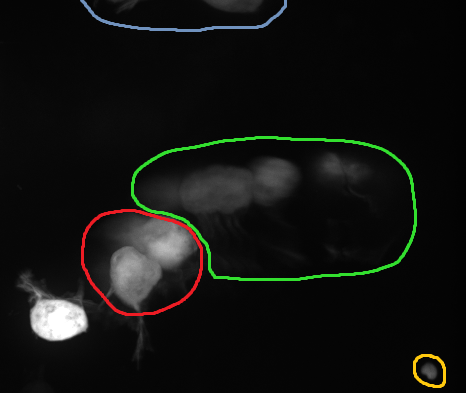
\includegraphics[scale=0.55]{img/fig_problems.png}
	\end {subfigure}
	\hspace{1cm}
	\begin {subfigure}[t]{0.40\linewidth}
		%\textbf{TODO: Uncomment this}
		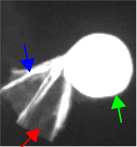
\includegraphics[scale=1.470]{img/fig_cell_example.png}
	\end {subfigure}

	\caption[Segmentation challenges and cell parts.]{\textbf{Left:} Cropped part of a microscopy image, showing challenges segmentation algorithms must overcome: Obscured borders due to cell overlap (red), movement blur (green), clipped cells on the borders of the image (blue) and ``ghost cells'' from an image lower in the stack (orange). Additionally, the illumination in the image varies massively from cell to cell and the contrast between Lamellipodia, Filopodia and the background is generally low. \textbf{Right:} A Drosophila cell. Contrast and brightness are enhanced for clarity. The green arrow shows the cell body, the red arrow shows the Lamellopodium and the blue arrow shows one of many Filopodia.}
	\label{fig:cell_example}
\end {figure}

\noindent The remainder of this thesis is structured as follows: In Chapter \textbf{\ref{chap:concepts}}, different approaches to the image segmentation problem are explained. The following Chapter \textbf{\ref{chap:network}} describes the architecture of a neural network that was designed with a focus on cell segmentation, and also describes the individual layer types, activation functions and loss functions the network uses. Then, in Chapter \textbf{\ref{chap:training}}, information about the data sets used for training and validating the network as well as information about data pre-processing, training parameters and optimization methods is given. In Chapter \textbf{\ref{chap:results}}, the hardware details of the training- and testing environment are listed and the results of all proposed approaches are compared to each other. In Chapter \textbf{\ref{chap:conclusion}}, a conclusion is derived from the achieved results and finally, Chapter \textbf{\ref{chap:futurework}} presents some ideas that were considered worth examining but went untested in the course of this thesis due to time constraints. 